
%%% Page size, margins & default style %%%%%%%%%%%%%%%%%%%%%%%%%%%%%%%%%%%%%%%%%

\documentclass[10pt, a5paper, twocolumn]{article}
\usepackage[top=1.2cm, bottom=1.5cm, left=1.2cm, right=1.2cm]{geometry}
\setlength{\columnsep}{1.2cm}
\pagestyle{empty}

%%% Typography, encoding & hyphenation %%%%%%%%%%%%%%%%%%%%%%%%%%%%%%%%%%%%%%%%%

\usepackage[T1]{fontenc}                    % output encoding
\usepackage[utf8]{inputenc}                 % input encoding
\usepackage[spanish]{babel}                 % text language
\usepackage{microtype}                      % improve kerning
\usepackage{paratype}                       % sans-serif font
\renewcommand{\familydefault}{\sfdefault}   % sans-serif by default
\usepackage{parskip}                        % removing default indentation

%%% Horizontal rule %%%%%%%%%%%%%%%%%%%%%%%%%%%%%%%%%%%%%%%%%%%%%%%%%%%%%%%%%%%%

\usepackage[svgnames]{xcolor}               % color definitions
\usepackage{tikz}                           % drawing tools
\tikzstyle{track}=[
    postaction={draw=FireBrick,densely dashed,line width=10pt},
    postaction={draw=Black,double distance=4pt,line width=1pt},
    postaction={draw=FireBrick,densely dashed,line width=4pt}]
\newcommand{\TRACK}{
    \medskip\begin{center}
        \begin{tikzpicture}\draw[track](0,0)--(5.2,0);\end{tikzpicture}
    \end{center}\medskip}

%%% First page %%%%%%%%%%%%%%%%%%%%%%%%%%%%%%%%%%%%%%%%%%%%%%%%%%%%%%%%%%%%%%%%%

\usepackage[10pt]{moresize}                 % \HUGE in the title
\usepackage{titling}                        % pretitle and postitle
\newcommand{\RULE}{\color{DarkRed}\rule{\linewidth}{1.5pt}}
\pretitle{\vspace{-25pt}\RULE\par\vspace{5pt}\HUGE\color{DarkRed}\begin{center}}
\posttitle{\end{center}\par\vspace{10pt}\RULE}

%%% Last page %%%%%%%%%%%%%%%%%%%%%%%%%%%%%%%%%%%%%%%%%%%%%%%%%%%%%%%%%%%%%%%%%%

\usepackage{fancyhdr}                       % custom headers and footers
\renewcommand{\headrulewidth}{0pt}          % remove header rule
\renewcommand{\footrulewidth}{1.5pt}        % draw footer rule
\fancyhf{}                                  % reset footer
\fancyfoot[R]{\footnotesize
\includegraphics[height=0.75em]{pic/cc.pdf}\,
\includegraphics[height=0.75em]{pic/by.pdf}\, {Carlos Luna Mota},\, \textit{\today}\,}

%%% Dialogue enviroment %%%%%%%%%%%%%%%%%%%%%%%%%%%%%%%%%%%%%%%%%%%%%%%%%%%%%%%%

\usepackage{enumitem}                       % custom description enviroment
\newenvironment{dialogue}
    {\begin{description}[leftmargin=!,align=right,labelwidth=0.cm]}
    {\end{description}}

\usepackage[tikz]{bclogo}                   % dialogue icons
\newcommand\A{\item[\raisebox{-0.25em}{\scalebox{0.75}{\bctetraedre}}]}
\newcommand\B{\item[\raisebox{-0.25em}{\scalebox{0.75}{\bccube}}]}
\newcommand\C{\item[\raisebox{-0.25em}{\scalebox{0.75}{\bcoctaedre}}]}
\newcommand\D{\item[\raisebox{-0.25em}{\scalebox{0.75}{\bcdodecaedre}}]}
\newcommand\E{\item[\raisebox{-0.25em}{\scalebox{0.75}{\bcicosaedre}}]}

%%% PDF's metadata %%%%%%%%%%%%%%%%%%%%%%%%%%%%%%%%%%%%%%%%%%%%%%%%%%%%%%%%%%%%%

\usepackage[pagebackref=false, hidelinks]{hyperref}
\hypersetup {
    pdfauthor    = {Carlos Luna Mota},
    pdfsubject   = {T3CS on rails},
    pdftitle     = {T3CS on rails},
    pdfkeywords  = {RPG, juego de rol, manual, actual play},
    pdfcreator   = {LaTeX},
    pdfproducer  = {pdflatex \& ghostscript}
}
\title{T3CS on rails}
\author{}
\date{}

%%%%%%%%%%%%%%%%%%%%%%%%%%%%%%%%%%%%%%%%%%%%%%%%%%%%%%%%%%%%%%%%%%%%%%%%%%%%%%%%

\begin{document}

    \maketitle\thispagestyle{empty} %%%%%%%%%%%%%%%%%%%%%%%%%%%%%%%%%%%%%%%%%%%%

    \begin{dialogue}
        \A Uff... casi no llegamos...
        \B Sí, ya podías haber mirado antes el número de andén...
        \A ¿Yo? ¡Si es por vosotras aún estamos en la otra punta!
        \E ¡Cabronas, anda que ayudáis con las maletas!
        \A Teníamos que coger mesa, que van a ser un montón de horas.
        \E Dejadme un asiento, anda, que estoy \emph{deslomá}.
        \A ¿Habéis traído cartas o algo?
        \B Yo no.
        \E Pues yo tampoco.
        \B ¡Pero si siempre las traes tú!
        \E Sí, pero hoy llevo la maleta grande y me las he dejado en la mochila.
        \A ¿Y qué hacemos? Tengo el móvil sin batería... y yo sentada no me duermo.
        \E No sé... Tú siempre estás diciendo que quieres jugar a rol con nosotras... podríamos echar una partida.
        \A ¿Aquí? ¿Quieres decir?
        \B ¿No has traído cartas y te traes el manual?
        \E Algo así... ¿Tenéis suelto?
        \B ¿Ahora cobras por dirigir?
        \A En serio ¿vais a poneros a jugar aquí en medio?
        \E Sí, y tú también. Y tranquila que no va a venir nadie a detenernos.
        \B Detenernos no sé, pero ahí viene el revisor y como no saquéis los billetes a lo mejor nos echa...
    \end{dialogue}

    \TRACK %%%%%%%%%%%%%%%%%%%%%%%%%%%%%%%%%%%%%%%%%%%%%%%%%%%%%%%%%%%%%%%%%%%%%

    \begin{dialogue}
        \E Bueno, esto ya se mueve, vamos al tajo ¿tenéis tres monedas?
        \A ¿Cómo las quieres? ¿Todas iguales?
        \E Me da igual, mientras nos pongamos de acuerdo en qué lado es cara y qué lado es cruz, me valen.
        \B Dale céntimos, que seguro que luego se los queda.
        \E Tu calla, que aún me debes las cervezas del otro día...
        \B ¡Hostia es verdad! Luego te las pago.
        \A Ten, tres monedas de 20 céntimos.
        \E Perfecto, Cervantes es cara y Europa es cruz ¿vale?
        \B ¿Pero a qué carajo vamos a jugar con tres monedas? 
        \E A lo que quieras... o, mejor dicho, a lo que tú quieras.
        \A ¿Yo? ¡Pero si no tengo ni idea!
        \E Precisamente. Dime una peli o una serie que te mole.
        \A ¿Vale cualquiera?
        \E La primera que te venga a la cabeza.
        \A No sé... ¿Perdidos?
        \B Que paren el tren, que me bajo...
        \E ¡Pero si nos enganchaste tú!
        \B Ya, pero el final... ese final no tiene perdón de Dios.
        \A Si queréis digo otra...
        \E No, da igual, la primera idea es la que vale. Y si la \emph{señora guionista} es tan lista como dice, seguro que estará encantada de arreglar la serie.
        \B Peor no va a quedar...
        \E Además, no se trata de jugar con los personajes o la trama de la serie, se trata de que nos pongamos de acuerdo en la situación inicial y juguemos para ver que pasa.
        \B ¿Eso no era lo de \emph{Apocalypse Now}?
        \E Es \emph{Apocalypse World}...
        \B Es que ya sabes que a mí los juegos \emph{indios} no me van mucho...
        \E No tiene por qué ser \emph{indie}... \emph{sandboxes} se han jugado toda la vida.
        \A Me estoy perdiendo.
        \E Sí, perdona, volvamos al tema. Perdidos sólo nos da un punto de partida y unas expectativas: gente atrapada en una isla desierta, sucesos paranormales, la \emph{Iniciativa Dharma}...
        \A El humo negro, osos polares, números chungos...
        \E Sí, también, pero no necesariamente todo a la vez. No se trata de repetir una parte de la serie...
        \B ¡Gracias a Dios!
        \E ...sino de coger esos ingredientes y crear una nueva historia con ellos.
        \A Uff... A mí estas cosas se me dan fatal.
        \E No te preocupes, es falta de práctica, nosotras te ayudamos.
        \B Tú fíjate en las \emph{pofecionaleh}...
        \E No lo dirás por ti, que aún me acuerdo de la partida de hace un mes...
        \B ¿Cómo iba a saber yo que ahí dentro cabía un dragón?
        \E En fin, a lo que vamos, ya tenemos la ambientación y el tono de la partida, ahora necesitamos personajes y una situación inicial interesante... ¿Ideas?
        \B Déjame que piense...
        \A Umm... ¿Vamos en un avión y nos estrellamos en una isla desierta?
        \E \emph{Back to basics}, me gusta, pero vamos a darle una vuelta de tuerca... ¿Qué os parece esto? ``Un mes después de la desaparición del vuelo de \emph{Oceanic Airlines}, la policía da por muertos a todos los pasajeros, pero vosotras os negáis a darlos por \emph{perdidos}...''
        \B Finísimo ese juego de palabras.
        \E ``...y decidís invertir todos vuestros ahorros en una misión de rescate. Tras semanas de sobrevolar la región en avioneta sin encontrar rastro alguno, una tormenta tropical amenaza con dar al traste con la búsqueda. Desesperadas porque se os está acabando el tiempo y el dinero, decidís arriesgar y salís a sobrevolar la última región que os quedaba por explorar. Lamentablemente, la tormenta os atrapa antes de que podáis regresar y un rayo deja frita la avioneta. Notáis una súbita ingravidez y veis al piloto luchar con los mandos mientras el copiloto intenta pedir ayuda por radio...''
        \B A mí me mola...
        \A A mí también, pero... ¿Te acabas de inventar todo eso?
        \E Sí, más o menos. Coges clichés del género, ideas sueltas, fragmentos de libros... lo mezclas todo y que sea lo que Dios quiera...
        \A Si tú lo dices...
        \E Ok, vamos a ver quienes sois y qué hacéis ahí... Empieza tú.
        \B Pues no sé... ya hemos dicho que conocemos a alguien del vuelo... Va, sí, lo veo... Me llamo Mike y mi mujer... Sara... iba en ese vuelo... y estaba embarazada así que estoy muy desesperado y he vendido la vieja granja de la familia para pagar esta misión de rescate.
        \E No sabe \emph{nah} la \emph{munchkin} esta...
        \B ¿\emph{S'ha notao}?
        \A ¿Qué me he perdido?
        \E No ha elegido un oficinista o un experto en literatura etrusca... Ha elegido un granjero porque alguien \emph{de campo} tiene más números de sobrevivir en una isla desierta.
        \A ¿Y eso es trampa?
        \E Mientras no sea muy forzado, no. De hecho es útil. ¿Por qué crees que el prota de Perdidos es precisamente un médico?
        \A Ostras, no lo había pensado nunca...
        \B Esa es la gracia de jugar a rol. Yo a veces veo pelis y pienso: ese personaje acaba de fallar una tirada.
        \E O cuando Gandalf saca un crítico y se carga al Balrog con el bastón...
        \A Si habláis raro no me entero.
        \E Tienes razón. Va, te toca, ¿quién eres y a quién estás buscando?
        \A ¿Yo no busco a Sara?
        \E No, casi mejor que tú vayas a buscar a otra persona.
        \A ¿Por?
        \E Así puedo meter cizaña entre vuestros personajes...
        \B No sabe \emph{nah} la \emph{munchkin} esta...
        \E \emph{Touché}...
        \A ¿Pero entonces qué hacemos juntos?
        \B Estábamos en una taberna cuando se nos acercó un bardo que...
        \E No le hagas caso... Tras el accidente, las familias de las víctimas se agruparon en una asociación para demandar a \emph{Oceanic} y allí os conocisteis. Cuando se dio a los pasajeros por \emph{perdidos}...
        \B Va a ser así todo el rato, ¿verdad?
        \E Ya te digo... Cuando se dio a los pasajeros por \emph{perdidos}, Mike os propuso juntar vuestros ahorros para continuar la búsqueda, pero tu personaje fue el único que se apuntó. Y ahora... ¿Por qué se apuntó tu personaje?
        \A Pues... ¿No me lo puedes contar tú?
        \E Yo te ayudo, pero es tu personaje y tu historia.
        \A Ok, a ver, ya me diréis si lo hago mal ¿vale? Pues yo... yo soy Jessica y estoy buscando a mi hermano... ¿Robert?
        \E ¿Y a qué se dedica Jessica y por qué se ha apuntado a este rescate?
        \A Ummm... Robert y yo somos mellizos y estamos muy unidos... Cuando le pasa algo malo puedo sentirlo como si me pasase a mí y por eso sé que está vivo: no he sentido su muerte.
        \B A lo mejor está fuera de cobertura...
        \E Tu calla, que se lo está currando... ¿De dónde has sacado el dinero?
        \A Nuestro padre era muy rico, hemos heredado mucho dinero.
        \E Ok, me va bien que tu personaje sea un poco pijete. Podrías ser la abogada que ha montado la asociación de víctimas...
        \A Pero entonces no sabré nada de sobrevivir en la isla.
        \E Ningún problema, no hace falta que todos los personajes sepan de todo. De hecho, mejor si cada uno cubre un tema diferente: Mike se ocupa de la supervivencia y tú puedes resolver enigmas o descifrar códigos...
        \A ¡Mola!
        \E Una última cosa... Has dicho que habéis heredado... Deduzco que tus padres está muertos.
        \A Sí, mamá murió en el parto y papá cuando teníamos 20 años. Robert lo llevó fatal y yo tuve que ser la responsable.
        \E Perfecto, me estás dando material para días...
        \A Si tú lo dices...
        \E Ya lo irás viendo... Recapitulemos: Mike es un granjero que lo ha hipotecado todo para rescatar a su mujer Sara, que está embarazada. Jessica es una abogada con mucha pasta que va a rescatar a su hermano mellizo Robert, con el que tiene una conexión especial y del que se siente responsable... Cuando sobrevuelan la región donde desapareció el vuelo de \emph{Oceanic Airlines}, una tormenta los atrapa y un rayo los hace caer... Sí, creo que ya tenemos todo lo que necesitamos para empezar...
        \A Ah, ¿pero no habíamos empezado todavía?
        \E No, todo eso era la preparación de la partida.
        \A No me extraña que os paséis tantas horas jugando a rol...
        \E De hecho, ahora que lo dices, creo que voy al lavabo para no tener que levantarme luego.
        \A Yo también.
        \E Luego me paso por el vagón restaurante a pillar algo para comer y beber. ¿Qué os traigo?
        \B Ya voy yo y así compenso las cervezas del otro día.
        \E Pues tráeme una coca-cola zero y una bolsa de patatas.
        \B ¿Y para ti?
        \A Lo mismo.
    \end{dialogue}

    \TRACK %%%%%%%%%%%%%%%%%%%%%%%%%%%%%%%%%%%%%%%%%%%%%%%%%%%%%%%%%%%%%%%%%%%%%

    \begin{dialogue}
        \E Bueno, vamos al lío.
        \B Faltan las fichas de personaje ¿no?
        \E No, no hacen falta, vamos a usar un sistema muy ligero. \textbf{Cuando toque hacer una tirada sólo hay que decidir si la cosa está 50$\!$\%---50$\!$\% o si el personaje tiene algún tipo de ventaja o desventaja}.
        \B ¿Y eso lo decides tú a ojo?
        \E En realidad no. \textbf{Si todas las demás estamos de acuerdo en que tu personaje tiene ventaja o desventaja, la tiene y no hay más que hablar}. \textbf{Si no nos ponemos de acuerdo, entonces se hace la tirada por defecto, que es la de 50$\!$\%---50$\!$\%}.
        \B ¿Y yo no pinto nada?
        \E \textbf{Quien lleva el personaje puede argumentar, pero no tiene voto}.
        \B No sé... esto de jugárselo todo a cara o cruz es un poco ir a lo loco... ¿Si intento volver a casa nadando también tengo un 50$\!$\%---50$\!$\% de conseguirlo?
        \E ¿De verdad necesitas reglas para saber que volver a casa nadando es mala idea?
        \B No, supongo que...
        \E Pues tú confía en mí, que sé lo que me hago. Cuando estés metida en la partida no te vas a dar cuenta de qué sistema estamos usando.
        \A Me estoy perdiendo un poco, me podéis explicar como va el tema este de las tiradas.
        \E No te preocupes, la primera escena la hago sólo con Mike y así ves cómo funciona.
        \A Vale.
        \E Vamos a empezar... Mike, recuperas poco a poco la consciencia. Delante de ti, centenares de hojas bailan rítmicamente. Sientes náuseas y todo te da vueltas. Notas el cuerpo magullado y una fuerte presión en el abdomen. Cuando por fin consigues enfocar correctamente la mirada, ves que hay un árbol dentro de la avioneta. Confuso, miras a derecha y a izquierda y ves a Jessica desmayada en su asiento. Está doblada por la cintura como una muñeca de trapo. Lentamente todo empieza a tener sentido. La avioneta se ha partido por la mitad. La cola, que es donde estáis, está reposando precariamente sobre la copa de un árbol. La presión que sientes es en realidad tu cinturón de seguridad, que ahora mismo es lo único que te mantiene unido al asiento. Notas cómo la avioneta, o lo que queda de ella, se balancea y no sabes dónde, pero el olor a humo te indica que en alguna parte hay algo ardiendo. ¿Qué haces?
        \B Cagarme en la \emph{máster}.
        \E Vale, ¿pero qué hace tu personaje?
        \B A ver, por partes, ¿veo alguna rama a la que me pueda coger o algo?
        \E Tienes que imaginarte que sólo queda la parte de cola del avión, justo por detrás de las alas. Vuestros personajes estaban sentados en la última fila y todo lo que tenían por delante ha desaparecido. Os aguantáis entre las copas de dos o tres árboles. El que tenéis delante frena la caída del avión mientras que los otros elevan el timón de popa hacia el cielo. Si te agarras fuerte al respaldo de tu asiento puedes desabrocharte el cinturón, pero para pasar al árbol tienes que saltar y vas a tener que hacer una tirada.
        \B Ok, me hago una idea. ¿Ella está inconsciente?
        \E Sí, la llamas y no responde.
        \A Siempre duermo profundamente...
        \B Vale. ¿A qué altura estamos? ¿Veo alguna cuerda o algo con la que la pueda atar para bajarla del avión?
        \E Estáis a unos 4 metros. No ves nada que te permita atarla.
        \B Me lo estás poniendo difícil.
        \E Es que tú ya sabes de qué va esto y quiero ver qué se te ocurre.
        \B Ok, \emph{challenge accepted}, ¿qué veo a mi alrededor?
        \E Ves la poca carga que llevabais totalmente revuelta. Un par de maletines de color naranja, un petate de lona, tres chalecos salvavidas, una lata de gasolina atada a la pared, ...
        \B Vale... creo que lo tengo. Me agarro al respaldo de mi asiento y me quito el cinturón.
        \E Ok, desde ahí puedes alcanzar los objetos que te he dicho o moverte al respaldo de su asiento.
        \B Miro los objetos para ver si hay algo de utilidad.
        \E Uno de los maletines tiene una pistola de bengalas y el otro es un botiquín. El petate está vacío y la lata de gasolina está llena.
        \B Ok, meto los maletines y la lata de gasolina en el petate y me lo pongo a los hombros.
        \E Hay humo, no sabes dónde está el fuego y te pones una lata de gasolina a la espalda... Va a ser una partida muy corta...
        \A Voy a morir antes de empezar a jugar, ¿verdad?
        \E De hecho, en \emph{Traveller} un personaje puede morir antes de...
        \B Vale, vale, cambio de planes. Saco la lata del petate y la tiro fuera del avión. Esperemos que aguante...
        \E Ahí, a lo loco...
        \B Con el petate puesto, cojo los chalecos salvavidas y me muevo al respaldo de su asiento.
        \E Creo que veo por donde vas. El avión se balancea con tus movimientos y cada vez hay más humo, pero consigues ponerte detrás de su asiento.
        \A Bua... me estoy poniendo nerviosa.
        \B Le pongo un chaleco alrededor del torso, dejando los brazos por dentro, y el otro alrededor de la cabeza.
        \A ¿Cómo?
        \B Me pongo el tercer chaleco salvavidas y tiro de las anillas para inflar los tres chalecos. Abro su cinturón de seguridad intentando dirigir la caída lo mejor que puedo.
        \A ¡Que no soy una lata de gasolina!
        \B ¡Por eso te he puesto los chalecos!
        \E Hola, mi nombre es Mike y esto es \emph{Jackass}... Bien, haces todo lo que has dicho y dejas que su cuerpo se deslice hasta el borde del fuselaje. Desde allí lo dejas caer y, aunque no puedes ver cómo ni dónde ha caído, escuchas como golpea dos o tres ramas antes de detenerse en el suelo con un PLOFFF.
        \B ¡Bien!
        \A ¿Bien?
        \E Cada vez te es más difícil respirar por culpa del humo. ¿Qué haces?
        \B Busco la mejor manera de saltar y agarrarme al árbol en plan bombero.
        \E Vale pues me vas a hacer una tirada para ver cómo va el tema. Yo creo que entre el petate, el chaleco inflado y que acabas de sobrevivir a un accidente aéreo, la tirada debería ser con desventaja. ¿Tú qué opinas?
        \A ¿Yo? ¿Y yo qué sé lo que es ventaja o desventaja?
        \E \textbf{Un personaje tiene ventaja cuando es imposible que lo que intenta salga totalmente mal}. Quizá no consigue lo que quiere conseguir, pero en todo caso no será un completo desastre. Con desventaja es lo mismo, pero al revés: \textbf{Un personaje tiene desventaja si es imposible que le salga todo como querría}. Quizá lo consiga, pero algo tendrá que pagar a cambio.
        \A Visto así... y teniendo en cuenta que me acaba de tirar como a un vulgar saco de patatas... Yo también creo que tiene desventaja.
        \B De desagradecidas está el mundo lleno... Vale, desventaja, no voy ni a discutir. ¿Qué tiro?
        \E \textbf{Por defecto, tirarías tres monedas y contarías las caras, pero con ventaja o desventaja sólo se tiran dos}.
        \B En serio, te estás inventando las reglas sobre la marcha, ¿no?
        \E No, es un sistema para improvisar partidas que encontré por internet. Se llama \textbf{T3CS}.
        \B ¿\emph{Text}?
        \E No, \textbf{T3CS}, las siglas de \emph{The 3 Coins System}, pero pronunciando el 3 como si fuese una ``E''.
        \B Muy \emph{original} el nombre... No lo había oído nunca.
        \E No es muy conocido, pero va bien cuando vas de viaje. Una vez lo jugué con chapas de cerveza en un bar.
        \A Hablando de jugar...
        \E Sí, venga, al tajo, tira dos monedas.
        \B Voy... una cara y una cruz.
        \E Ok, \textbf{si tiras con ventaja, la tercera moneda cuenta como una cara, mientras que si tiras con desventaja, cuenta como una cruz}. En este caso la tirada te queda con \textbf{una cara y dos cruces, que es un fallo parcial}, y lo narras tú.
        \B ¿Yo?
        \E Sí, \textbf{quien lleva el personaje narra los éxitos totales y los fallos parciales y quien dirige narra los éxitos parciales y los fallos totales}.
        \B Estos juegos \emph{modehnoh}... ¿Y puedo narrar cualquier cosa?
        \E Si te lo paras a pensar, es la manera natural de repartirlo... Y sí, puedes narrar lo que quieras, siempre que se pueda considerar un fallo parcial y sea coherente con lo que se ha dicho hasta ahora.
        \B Ok, a ver qué te parece esto: Salto del avión y pero fallo a la hora de agarrarme al tronco del árbol en plan bombero porque el chaleco está inflado y me hace rebotar. Caigo dándome de hostias con las ramas, pero el chaleco y el petate amortiguan un poco la caída y no me hago mucho daño.
        \E Si te haces un esguince o te cargas uno de los maletines, te lo compro.
        \B Uff... venga, se rompe el de las bengalas durante la caída.
        \E Ok, sigues teniendo las bengalas, pero la pistola se ha roto y no tienes manera de lanzarlas. Tu \emph{salto ninja} ha desestabilizado el fuselaje, que cada vez se balancea más. ¿Qué haces?
        \B La busco a ella y nos aparto de la trayectoria.
        \A ¡Ya era hora!
        \E La encuentras a un par de metros. Parece que los chalecos han amortiguado también su caída, porque respira con normalidad y no tiene heridas visibles, pero sigue inconsciente. La arrastras hasta un claro cercano.
        \B Ok, miro a ver si hay algo en el botiquín que me permita despertarla.
        \E En el botiquín hay muchas cosas. Mientras lo revisas, Jessica empieza a toser y balbucear.
        \B La intento reanimar.
        \E Recuperas la consciencia. Estás en medio de la selva y no tienes ni idea de lo que ha pasado. Te duele todo y estás desorientada. ¿Qué haces?
        \A Le pregunto qué ha pasado.
        \B Le explico lo que sé.
        \E Perfecto, estáis en medio de un bosque tropical. Debe ser media tarde y está nublado, pero no tiene pinta de llover en breve. Lo único que tenéis es lo que llevabais puesto y el petate con un botiquín y las bengalas.
        \B Cojo los chalecos y busco la lata de gasolina.
        \E Encuentras la lata de gasolina. Tiene una pequeña fisura por la que gotea la gasolina poco a poco, pero sigue bastante llena. 
        \B ¿La puedo meter en el petate sin que lo moje todo de gasolina?
        \E Si vas con cuidado y no haces el cabra, sí. En pocas horas anochecerá. ¿Qué hacéis?
        \A ¿Se ve de dónde veníamos?
        \E El rastro de árboles rotos os indica que veníais del norte. Mirando en dirección contraria podéis ver una columna de humo a lo lejos.
        \A ¡La otra mitad! ¡Vamos a investigar!
        \B Lo suyo sería prepararnos para la noche, pero quizá podamos encontrar cosas útiles antes de que se quemen.
        \E Vale, ¿os dirigís al sur?
        \B Sí, voy delante abriendo paso.
        \E Se me ha acabado la coca-cola y es un buen momento para parar la partida. ¿Os traigo algo?
        \B Yo estoy bien, pero aprovecho para ir al lavabo.
        \A ¿Hay magdalenas?
        \B Creo que sí.
        \A ¿Me traes una?
        \E Vale, ahora vuelvo.
    \end{dialogue}

    \TRACK %%%%%%%%%%%%%%%%%%%%%%%%%%%%%%%%%%%%%%%%%%%%%%%%%%%%%%%%%%%%%%%%%%%%%

    \begin{dialogue}
        \E ¿Por dónde íbamos?
        \A Estamos yendo a buscar la otra mitad de la avioneta.
        \E Ah, sí, llegáis al anochecer. El camino era difícil al principio, pero poco a poco la vegetación se hace menos densa y el bosque deja paso a una pradera. Eso es lo que os permite encontrar el avión aún después de que el humo haya cesado y el Sol empiece a ponerse. Encontráis la mitad delantera de la avioneta parcialmente calcinada. En su interior están los cuerpos del piloto y el copiloto... o lo que queda de ellos.
        \A ¿Había alguien más en la avioneta?
        \E No, sólo vosotros cuatro.
        \B ¿Hay algo que podamos aprovechar?
        \E Está todo en muy mal estado. Lo que no se ha quemado tras el accidente se había fundido por culpa del rayo.
        \B Al menos podemos usar el avión para pasar la noche, ¿no?
        \A ¿Con los muertos?
        \B No sabemos dónde estamos ni qué nos puede pasar si dormimos al raso. Y es tarde para montar un refugio.
        \A ¿Y no podemos enterrarlos o algo?
        \B ¿Tengo pinta de llevar una pala?
        \A Pues menudo granjero de pacotilla...
        \E Total, ¿qué hacéis?
        \B Nos resguardamos en lo que queda de la avioneta.
        \A Qué remedio...
        \E Ok, cae la noche y baja la temperatura. Os resguardáis del frío en la avioneta. No es cómodo, pero el cansancio os puede y, cuando se pasa el efecto de la adrenalina, caéis en un profundo sueño. A la mañana siguiente os despiertan los primeros rayos de Sol. Después de la desorientación inicial, os ponéis en pie. Vuestros cuerpos están entumecidos y tenéis sed. ¿Qué hacéis?
        \B Vuelvo a revisar la avioneta por si encuentro algo de utilidad ahora que hay más luz.
        \E Sigues sin encontrar nada.
        \A Yo creo que deberíamos enterrar al piloto y al copiloto.
        \B Es mucho trabajo... deberíamos encontrar agua y comida primero.
        \A Me pongo a cavar yo sola.
        \E Es una pradera... ¿Cómo lo haces?
        \A Busco algo que me sirva de pala.
        \E Ok, digamos que hay trozos de chapa de la avioneta por ahí tirados. ¿Y tú qué haces?
        \B Paso de discutir. Le digo que voy a explorar los alrededores para buscar agua y que no se mueva de ahí hasta que vuelva.
        \E Perfecto. Pues das una vuelta por la pradera y te internas un poco en el bosque. Hazme una tirada para ver qué encuentras.
        \B Con ventaja por ser granjero, ¿no?
        \E Venga, te lo compro.
        \B ¿Dos monedas también?
        \E Sí, pero pon la sudadera en la mesa, que así hacemos menos ruido.
        \B Ok, tiro y... una cara y una cruz.
        \E Como tirabas con ventaja, la tercera moneda también cuenta como una cara y te quedan \textbf{dos caras y una cruz, que es un éxito parcial}, y me toca narrar a mí. Veamos... No encuentras ningún riachuelo, pero reconoces algunas lianas que quizá tengan algo de agua en su interior. Intentas beber de ellas, pero son demasiado correosas y no puedes cortarlas a mano.
        \B Busco una piedra afilada o algo.
        \E ¿En plan neanderthal?
        \B Vale... pues vuelvo a la avioneta para buscar algo que me pueda servir de machete y para decirle a ella que he encontrado agua.
        \E Presuntamente...
        \B Lo que sea.
        \E Vuelves a media mañana y la encuentras medio desmayada en la avioneta. Ha estado trabajando a pleno sol y está bastante deshidratada.
        \A ¡Siempre me toca pringar!
        \E Las decisiones que tomas tienen consecuencias.
        \B ¿Puedo llevarla a donde he encontrado las lianas?
        \E Sí, la abanicas un poco y se recupera.
        \B ¿Encuentro algo que me sirva de machete?
        \E El trozo de chapa que ha usado para cavar las tumbas del piloto y el copiloto está un poco afilado.
        \B Pues cojo la chapa y nos ponemos en marcha a las lianas.
        \E Al salir de la avioneta te parece ver algo a lo lejos. Un parpadeo.
        \B ¿Un animal?
        \E No estás seguro porque lo has visto de refilón, pero no, no parecía un animal. Dirías que era un destello y provenía de una montaña no muy alta que hay en dirección norte.
        \B ¿Un faro? ¿Un rayo? ¿Fuego?
        \E No lo sabes. Ahora no ves nada.
        \A ¿Yo veo algo?
        \E Él te explica lo que ha visto y te indica más o menos de dónde provenía.
        \B Nos quedamos un rato mirando en aquella dirección.
        \E Hacedme una tirada a ver si conseguís volverlo a ver. Como lo estáis buscando, os dejo tirar con ventaja.
        \B ¿Tiramos las dos?
        \E No, una tirada en total, parte de la ventaja es que mirais a la vez.
        \A Tiro yo, que aún no he tirado. Dos monedas, ¿verdad?
        \E Sí.
        \A Pues... ¡dos caras!
        \B A partir de ahora tiras siempre tú.
        \E Teneis un total de \textbf{tres caras, que és un éxito total}, y en teoría deberíais narrar vosotras, pero como no sabéis lo que estáis mirando, si os parece, narro yo.
        \A ¡Cuenta, cuenta!
        \E Pues... después de un buen rato lo veis otra vez, esta vez con mucha más claridad. Es un destello muy breve y por la posición del Sol deducís que debe ser un rayo de luz reflejado en alguna superficie muy pulida. Está justo encima de un saliente de roca de la montaña, así que no os costará localizarlo de nuevo en el futuro.
        \A Quizá sea un edificio o algo.
        \B Habrá que ir a investigar... Con la pala improvisada hago una flecha en la pradera señalando la dirección en la que hemos visto el destello por si alguien viene a rescatarnos y encuentra la avioneta.
        \E ¿Cómo que \emph{hago una flecha}?
        \B Cabo unos surcos grandes que se vean desde el aire.
        \E Ah, vale. ¿Algo más?
        \A ¡Vamos a investigar los destellos!
        \B Sí, pero primero cojo el petate y la pala y nos desviamos a beber agua de las lianas.
        \A ¡Aburrida!
        \E Vale, las lianas no son ninguna maravilla, pero os hidratan, que es lo importante. La sombra del bosque también se agradece y empezáis a sentiros mejor. La pala en manos de Mike sirve para abriros paso entre la vegetación, pero aun así tardáis casi todo el día en llegar al pie de la montaña y empieza a oscurecer. ¿Qué hacéis?
        \A ¿Hay alguna cueva o algo por aquí?
        \E Exploráis un poco los alrededores en busca de una cueva. Hay poca luz y tropiezas con algo. Al principio piensas que es una rama, pero en seguida os dais cuenta de que se trata de un cable bastante gordo. ¿Qué hacéis?
        \B ¡Lo seguimos!
        \E ¿En qué sentido?
        \B De momento hacia la montaña.
        \E Seguís el cable con bastante dificultad hasta una pared de roca. Justo al lado de donde el cable entra en la pared hay una cueva. No parece una formación natural, es como si alguien la hubiese excavado. ¿Entráis?
        \A ¡Claro!
        \B ¡No tan rápido! ¿Cómo es la cueva? ¿Podemos ver lo que hay dentro?
        \E Cada vez hay menos luz y no veis los detalles, pero no parece muy profunda y al fondo veis lo que parece ser una lucecita muy tenue.
        \B Voy delante usando la pala de escudo.
        \A ¿Quieres decir que hace falta?
        \B A mí no me vuelve a pillar un dragón por sorpresa...
        \E Vais a tientas, pero el suelo es bastante regular y os adentráis 5 o 6 metros en lo que a todas luces es un túnel artificial. Al fondo hay una puerta metálica y panel retroiluminado. El panel tiene un teclado numérico y en la pantalla veis que el código es de 6 cifras agrupadas de 2 en 2.
        \B ¡No vamos a acertar 6 cifras nunca!
        \A ¿Y si picamos a la puerta?
        \E Picáis una y otra vez, pero nadie contesta ni os abre. Todo parece indicar que no hay nadie al otro lado.
        \B ¿Podemos ir probando códigos hasta que se abra?
        \E No parece haber un número máximo de intentos, pero con 6 cifras hay un millón de posibilidades...
        \B Yo voy probando igualmente.
        \A ¿No debería probar yo? ¿Antes has dicho que Jessica era la que iba a hacer estas cosas?
        \E Sí, de hecho tú te fijas en que algunas teclas están un poco más desgastadas que otras... Es más, son cifras que, en cierto orden, tienen un significado especial para ti: Es la fecha en la que nacisteis Robert y tú.
        \A ¿Pruebo esa combinación?
        \B No perdemos nada...
        \E Marcas las 6 cifras de tu cumpleaños y oís como la puerta se desbloquea...
        \A ¡Mooola!
        \E ...pero hay un detalle más: Cuando te ve introducir el código, Mike también reconoce esas cifras... ¡Es la fecha de nacimiento de Sara!
        \B ¡Vamos que nos vamos!
        \E ¿Entrais?
        \A ¡No, si te parece nos quedamos fuera!
        \E Vale, pero necesito un respiro para coger ideas. Voy a estirar las piernas y a pensarme cómo seguimos.
        \B Ok, aquí te esperamos.
        \A ¡No tardes!
    \end{dialogue}

    %\TRACK %%%%%%%%%%%%%%%%%%%%%%%%%%%%%%%%%%%%%%%%%%%%%%%%%%%%%%%%%%%%%%%%%%%%%


    \TRACK %%%%%%%%%%%%%%%%%%%%%%%%%%%%%%%%%%%%%%%%%%%%%%%%%%%%%%%%%%%%%%%%%%%%%

    \begin{dialogue}
        \E Volvemos al tema, que creo que ya sé por donde tirar. Ibais a entrar, ¿no?
        \B Sí. Voy delante y llevo el escudo listo.
        \E Entrais a un pasillo y unos sensores de movimiento van activando los flourescentes conforme avanzais. Llegais a unas escaleras que suben y no hay más opciones, así que subís los dos primeros tramos. Allí encontrais una puerta. Podéis entrar o podéis seguir subiendo por las escaleras.
        \B ¿La puerta está abierta?
        \E Está cerrada, pero no tiene ningún tipo de cerradura. ¿La abres?
        \A ¿Hay algún cartel?
        \E Pues sí. Hay un cartel justo al lado de la puerta y otros dos señalando en cada sentido de la escalera. Lamentablemente... están en cirílico.
        \A Pero Jessica es muy lista, ¿no? ¡Seguro que sabe algo de ruso!
        \E Si me justificas cómo aprendió ruso, a lo mejor te lo compro.
        \A Pues Jessica habla ruso porque... porque... ¡sus abuelos maternos escaparon de la URSS en plena Guerra Fría!
        \E Aprende rápido la \emph{munchkin} esta...
        \B Ya te digo...
        \A ¿Eso es un sí?
        \E Sí, no tenía previsto hacer un \emph{crossover} con \emph{The Americans}, pero la verdad es que lo de tus abuelos rusos me ha molado. Digamos que sabes ruso pero lo tienes bastante oxidado porque tu madre murió en el parto y has tenido menos contacto con esa mitad de la família.
        \A ¡Vale!
        \B ¿Qué pone en los carteles?
        \E Pues te cuesta un poco, pero deduces que dicen: \emph{salida}, el que va hacia abajo; \emph{almacén}, la puerta que tenéis delante; y \emph{dormitorios}, \emph{comedor} y \emph{sala de control}, el que va hacia arriba.
        \B ¿Se oye algún ruido?
        \E Está todo en silencio como si no hubiese nadie.
        \B Será mejor que subamos directamente a la sala de control. A lo mejor hay alguna radio.
        \A ¿No deberíamos ir mirando planta por planta?
        \B Estamos en una isla tropical en la que hay una base excabada en la montaña con letreros en ruso. O es una instalación muy vieja, y está avandonada, o es una instalación muy secreta, y no les va a hacer gracia vernos. En cualquier caso prefiero no encontrarme a nadie.
        \A Visto así...
        \E Vais subiendo y encontrais tres plantas más: los dormitorios, el comedor y la sala de control. ¿Entrais?
        \B Abro la puerta un poco, ¿veo algo?
        \E Al abrir la puerta se encienden los fluorescentes de esa planta.
        \A Eso es que no hay nadie, ¿no?
        \E Veis un pasillo con varias puertas con letreritos. Parecen despachos.
        \B
        %
        %
        %
        \newpage
        \E ¿Os parece que lo dejemos aquí?
        \A ¿Ahora? ¡Pero si acabamos de abrir la puerta! ¡Yo quiero saber cómo acaba todo esto!
        \E Precisamente. Siempre es bueno dejar la sesión en un \emph{cliffhanger} para que no dé pereza volver a ponernos el próximo día. ¿Te ha gustado tu primera partida?
        \A ¡Mucho! ¿Podemos seguir a la vuelta?
    \end{dialogue}

    %\TRACK %%%%%%%%%%%%%%%%%%%%%%%%%%%%%%%%%%%%%%%%%%%%%%%%%%%%%%%%%%%%%%%%%%%%%


    \TRACK %%%%%%%%%%%%%%%%%%%%%%%%%%%%%%%%%%%%%%%%%%%%%%%%%%%%%%%%%%%%%%%%%%%%%

    \begin{dialogue}
        \E Bueno... ¿Qué os ha parecido?
        \B Me lo esperaba peor. Eso de jugarse las cosas a cara o cruz...
        \E Tú es que eres muy de BRP y D20, pero buena parte del \emph{crunch} de esos sistemas es ilusorio. Al final sólo hay cuatro resultados posibles: lo petas, lo consigues justito, fallas por poco o la cagas bien. Si hubiesemos jugado con otro sistema... ¿crees que la partida hubiese salido muy diferente?
        \B Supongo que no, al final eres tú la que ajusta las dificultades y tal... ¡pero las monedas ruedan menos que los malditos D4s!
        \E Ya, en casa lo juego con unos D6s educativos de sumas y restas.
        \B ¿Rollo dados Fate?
        \E Sí, pero sin caras en blanco, tres positivos y tres negativos. De todas maneras, va muy bien poder improvisarlo con monedas o lo que tengas a mano: Una vez le monté a mi sobrina una partida de iniciación y jugamos con conchas que habíamos recogido.
        \B Que hippy todo... y tu hermano sin sospechar que la estabas trayendo al \emph{lado oscuro}...
        \E Y, hablando de iniciación, ¿tú cómo lo has visto?
        \A A mi me ha parecido muy sencillo, pero es que yo no tengo ni idea y me iba dejando llevar. Al principio no me enteraba mucho, pero luego le he ido cogiendo el tranquillo...
        \E Los juegos de rol se aprenden jugando.
        \B O viendo jugar. Yo he aprendido algún sistema leyendo \emph{actual plays}.
        \E Sí, pero porque tú ya sabes jugar.
        \A Y... ¿Haremos otra partida?
        \E Tenemos todo el viaje de vuelta.
        \A ¡Pero queda mucho!
        \B La conversión se ha completado, tu alma nos pertenece, tu destino está ligado al gran \emph{Nyarlathotep}...
        \E No le hagas caso, podemos ir haciendo escenas sueltas cada vez que tengamos un rato suelto. Entre que no hay fichas de personaje y que usamos tres monedas, podemos jugar en el restaurante sin que nos miren raro.
    \end{dialogue}

    %%%%%%%%%%%%%%%%%%%%%%%%%%%%%%%%%%%%%%%%%%%%%%%%%%%%%%%%%%%%%%%%%%%%%%%%%%%%

    %\newpage

    %\hspace{0.1\textwidth}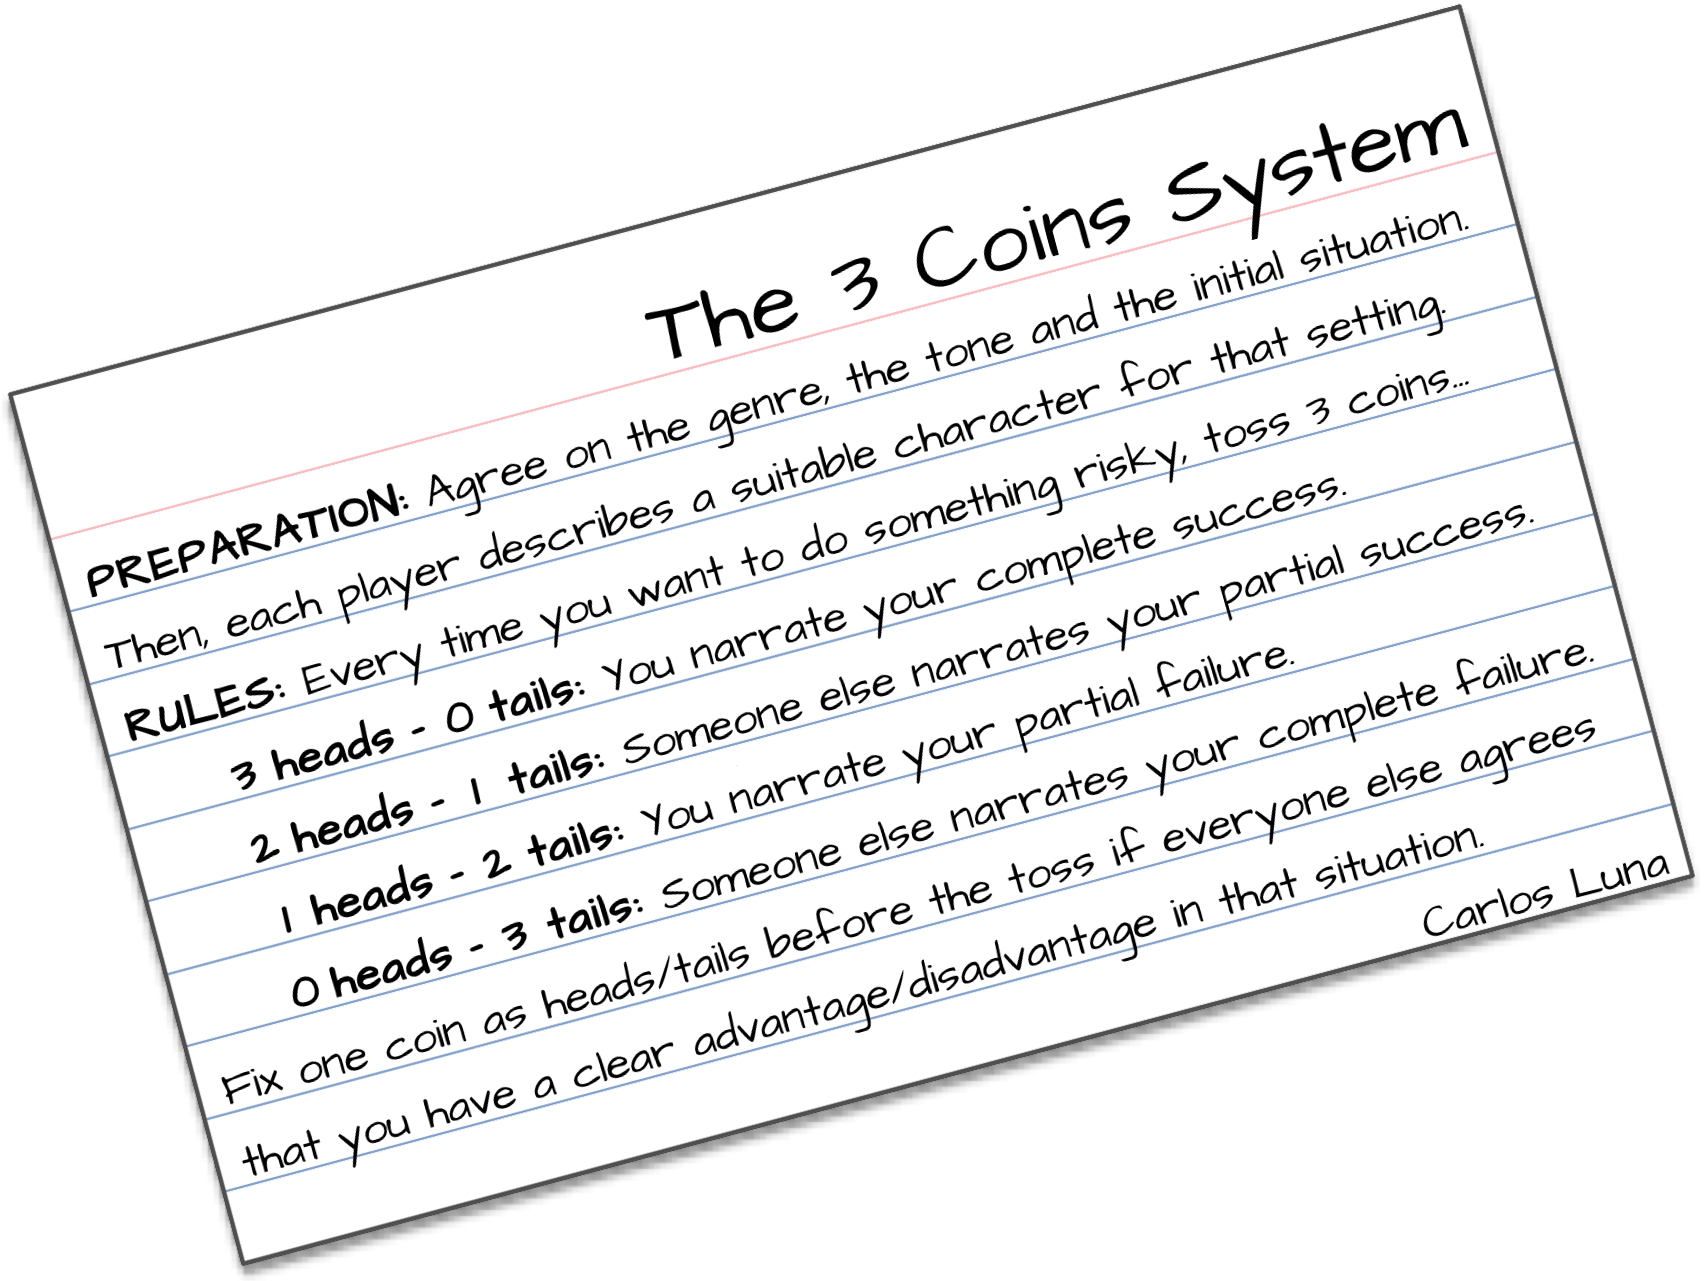
\includegraphics[width=0.8\textwidth]{pic/T3CS.png}
   
    \thispagestyle{fancy} %%%%%%%%%%%%%%%%%%%%%%%%%%%%%%%%%%%%%%%%%%%%%%%%%%%%%%

\end{document}

%%%%%%%%%%%%%%%%%%%%%%%%%%%%%%%%%%%%%%%%%%%%%%%%%%%%%%%%%%%%%%%%%%%%%%%%%%%%%%%%
